\todo{services.tex}

\subsection{Service Overview}

According to the manual FutureGrid provides a number of different
services. These services include:

\begin{enumerate}
\item OpenStack which includes a collection of open source components to deliver public and private clouds. These components currently include OpenStack Compute) OpenStack Object Storage, and OpenStack Image Service. OpenStack has received considerable momentum due to its openness and the support of companies. 

\item Nimbus which is an opensource service package that allows users to run virtual machines on FutureGrid hardware. Just as in Openstack users can upload their own virtual machine images or customize existing once. Nimbusnext to Eucalyptus is one of the earlier frameworks that make managing virtual machines easier.

\item Eucalyptus is an opensource software platform that implements IaaS-style cloud computing. Eucalyptus provides an Amazon Web Services (AWS) compliant EC2-based web service interface for interacting with the Cloud service.  Eucalyptus has been previously the dominant alternative to AWS  in academia. However, based on usage patterns in FutureGrid we believe it is replaced by OpenStack.

\item High Performance Computing can be defined as the application of supercomputing techniques to solve computational problems that are too large for standard computers or would take too much time. This is one of the more important features that the scientific community needs to achieve their projects. Naturally using HPC resouces and services is also useful in the area of Big Data. Sometimes big data needs big machines. Thus, using HPC may be an ovious choice.

\item Map Reduce …. TBD …

\end{enumerate}

Storage on FutureGrid has moderate size storage capability that will satisfy the users demand to compare and test someof the previously outlined services.

Information Services gather the information of the different elements that make up FutureGrid to provide accurate and complete knowledge of the computational environment. This information is presented using different web portals.

\begin{figure}[p]
  \centering
    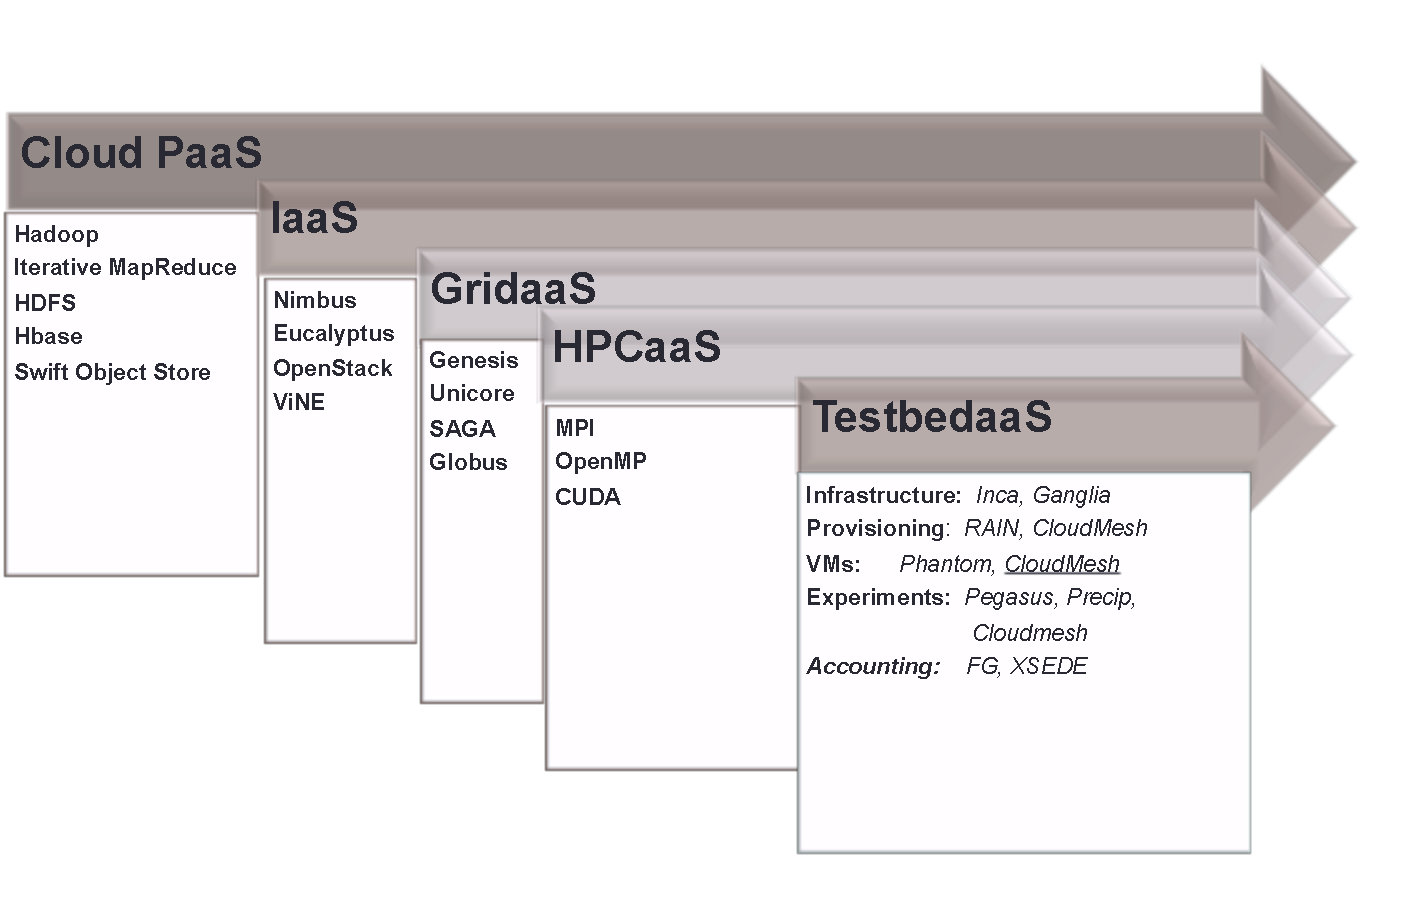
\includegraphics[width=0.9\textwidth]{images/user-services.pdf}
  \caption{FutureGrid High Level User Services.}
  ~\\
  \centering
  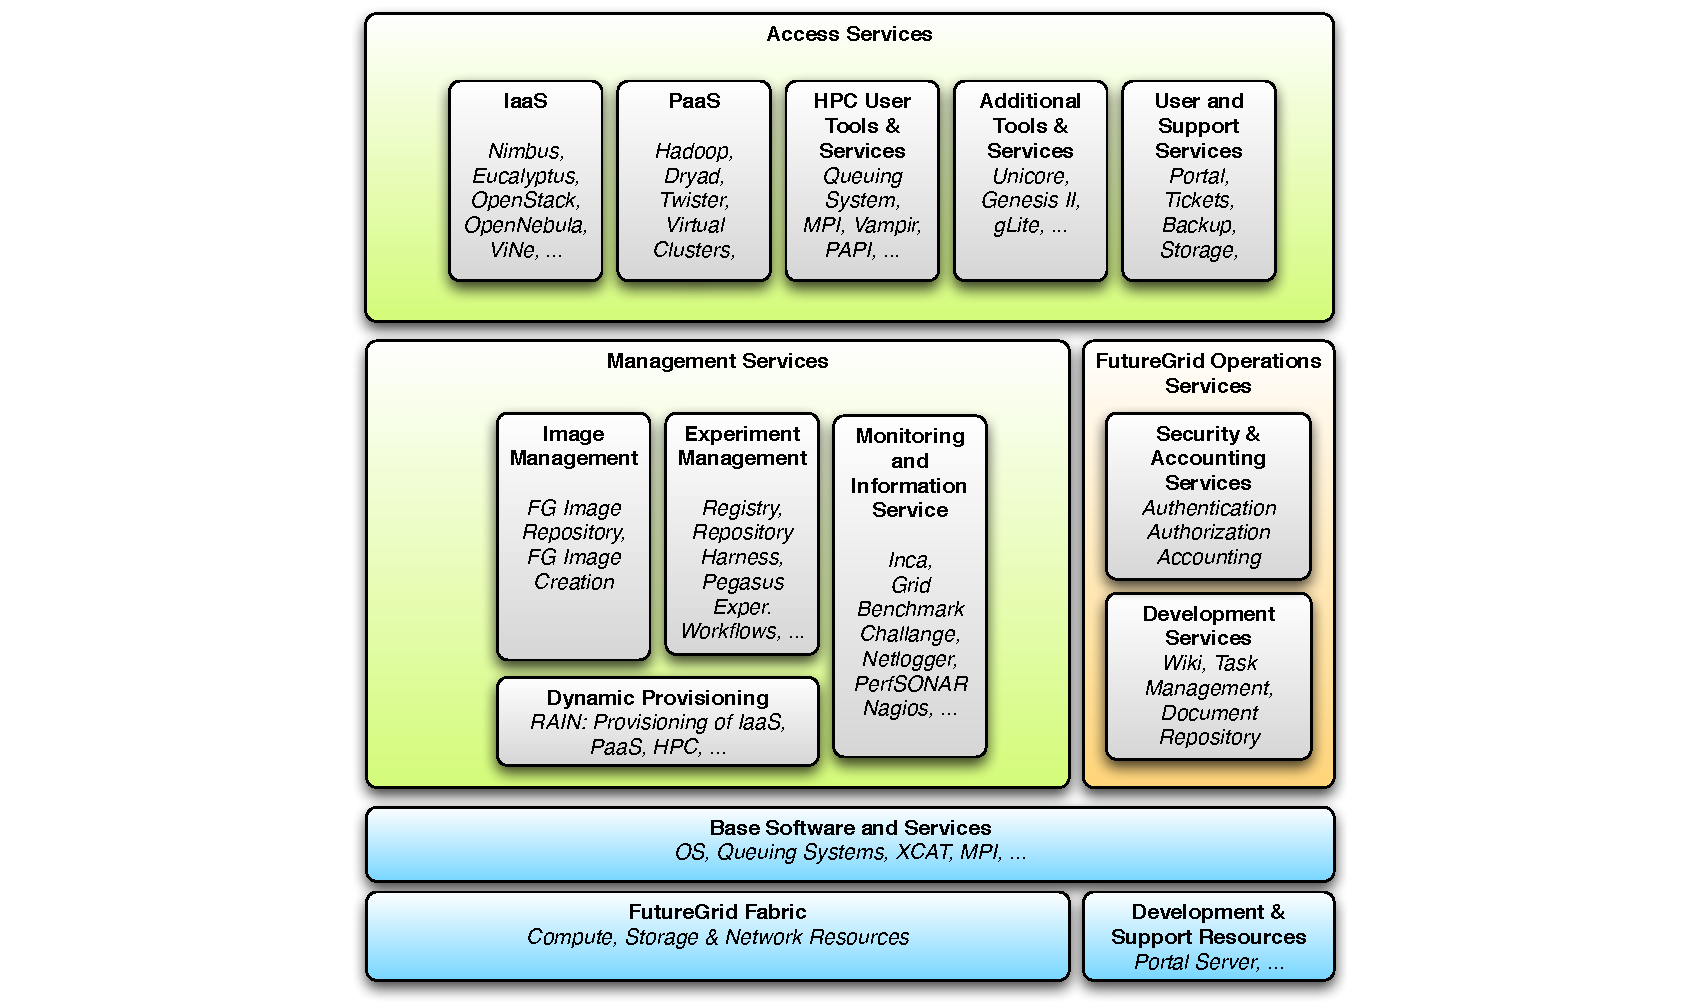
\includegraphics[width=0.9\textwidth]{images/architecture.pdf}
  \caption{Architecture.}
\end{figure}
